\documentclass[a4paper,oneside,12pt,pdftex]{article}
\usepackage[bahasa]{babel}
\usepackage[top=3cm,left=3cm,bottom=3.1cm,right=2cm]{geometry}
\usepackage{times}
\usepackage{graphicx}
\usepackage{wrapfig}
\usepackage{subfig}
\usepackage{array}
\usepackage{multirow}
\usepackage{color}
\usepackage{colortbl}
\definecolor{backgroundcolor}{rgb}{0.949019608,0.949019608,0.949019608}
\usepackage{hyperref}
\hypersetup{colorlinks,citecolor=blue,filecolor=black,linkcolor=blue,urlcolor= blue,breaklinks=true}
\usepackage{fancyhdr}
\pagestyle{fancy}
\fancyhead{}
\fancyfoot{}
\lfoot
{
\begin{tabular}{|>{\footnotesize}l|}
\hline
\cellcolor{backgroundcolor}Nomor Dokumen: PRO\hspace{1.6cm}Nomor Revisi: 05\hspace{0.7cm}Tanggal: 08/12/10\hspace{1.5cm}Halaman \thepage\hspace{3pt}dari 23\\
\hline
\end{tabular}\\
{\scriptsize\copyright 2010 oleh LSKK STEI-ITB. Pengungkapan dan penggunaan seluruh isi dokumen hanya dapat dilakukan atas ijin tertulis LSKK STEI-ITB Jalan Ganesha 10 Bandung, 40132 Indonesia.}
}
\renewcommand{\headrulewidth}{0pt}


\begin{document}

\addcontentsline{toc}{section}{Lembar Sampul Dokumen}

\begin{wrapfigure}{l}{0.125\textwidth}
\vspace{-0.5cm}

\includegraphics[height=2.6cm]{Ganesha}
%\rule{\linewidth}{0.2mm}
\end{wrapfigure}
\noindent\textbf{\textsf{\LARGE Dokumen Pengembangan Produk}}\\[0.8cm]
\textsf{\large LAB. SISTEM KENDALI \& KOMPUTER, STEI -- ITB}
\rule{\linewidth}{0.2mm}
\vspace{0.5cm}
\begin{center}
\textbf{\textcolor{sectioncolor}{\textsf{\large Lembar Sampul Dokumen}}}\\[1.1cm]
\end{center}

\arrayrulecolor{white}
\setlength\doublerulesep{11pt}

\begin{tabular}{p{4cm}>{\columncolor{backgroundcolor}}p{10.5cm}}
Judul Dokumen & DOKUMEN DESAIN PRODUK:\\[0.1cm]
 & \cellcolor{backgroundcolor}\emph{PUSPA}\\
\hline\hline
\end{tabular}

\begin{tabular}{p{4cm}p{10.5cm}}
Jenis Dokumen & \cellcolor{backgroundcolor}DSG: DESAIN PRODUK\\
 & \hspace{1.25cm}\textmd{\textsf{\scriptsize Catatan: Dokumen ini dikendalikan penyebarannya oleh LSKK, STEI -- ITB}}\\[0.4cm]
\end{tabular}

\begin{tabular}{p{4cm}p{10.5cm}}
Nomor Dokumen & \cellcolor{backgroundcolor}DSG\\
\hline\hline
\end{tabular}

\begin{tabular}{p{4cm}p{10.5cm}}
Nomor Revisi & \cellcolor{backgroundcolor} 02\\
\hline\hline
\end{tabular}

\begin{tabular}{p{4cm}p{10.5cm}}
Nama Berkas & \cellcolor{backgroundcolor}B300.pdf\\
\hline\hline
\end{tabular}

\begin{tabular}{p{4cm}p{10.5cm}}
Tanggal Penerbitan & \cellcolor{backgroundcolor}17 Maret 2010\\
\hline\hline
\end{tabular}

\begin{tabular}{p{4cm}p{10.5cm}}
Unit Penerbit & \cellcolor{backgroundcolor}PUSPA Dev Team\\
\hline\hline
\end{tabular}

\begin{tabular}{p{4cm}p{10.5cm}}
Banyak Halaman & \cellcolor{backgroundcolor}12\\
 & \\[1.1cm]
\end{tabular}

\arrayrulecolor{black}
\setlength\arrayrulewidth{1pt}

\begin{tabular}{|l|l|l|l|l|l|}
\hline
\multicolumn{6}{|l|}{\cellcolor{backgroundcolor}Data Pengusul}\\
\hline
Pengusul & Nama & \multicolumn{2}{l|}{Erik Prabowo} & Jabatan & \textit{Engineer}\\
 & & \multicolumn{2}{l|}{Rio Andita Setiabakti} & & \textit{Engineer}\\
\hline
\multicolumn{2}{|l|}{Tanggal} & \multicolumn{2}{l|}{17 Maret 2010} & Tanda &\\
\multicolumn{2}{|l|}{} & \multicolumn{2}{l|}{} & Tangan &\\
\hline
\multicolumn{2}{|l|}{Lembaga} & \multicolumn{4}{l|}{Rumah Tenda}\\
\multicolumn{2}{|l|}{} & \multicolumn{4}{l|}{Rakreasi}\\
\hline
\multicolumn{2}{|l|}{Alamat} & \multicolumn{4}{l|}{Jln. Ligar Kencana Blok B No. 8 Bandung 40191}\\
\multicolumn{2}{|l|}{} & \multicolumn{4}{l|}{Jln. Tubagus Ismail VIII No. 68 Bandung 40124}\\
\hline
Telepon & {\footnotesize 022-2509262} & Faks & {\footnotesize 022-2509262} & \textit{e-mail} & {\footnotesize\href{mailto:eprabowo@rumahtenda.web.id}{eprabowo@rumahtenda.web.id}}\\
 & {\footnotesize 022-82523428} & & {\footnotesize 022-82523428} & & {\footnotesize\href{mailto:rio.andita@gmail.com}{rio.andita@gmail.com}}\\
\hline
\end{tabular}

\vspace{0.75cm}

\arrayrulecolor{black}
\setlength\arrayrulewidth{0.6pt}

\tableofcontents
\addcontentsline{toc}{section}{\textcolor{black}{DAFTAR ISI}}
\part*{\textcolor{sectioncolor}{\textsf{\large Catatan Sejarah Perbaikan Dokumen}}}
\addcontentsline{toc}{section}{Catatan Sejarah Perbaikan Dokumen}

\begin{tabular}{|p{4cm}|p{11cm}|}
\hline
{\scshape Versi, Tgl, Oleh} & {\scshape Perbaikan}\\
\hline
01, 18 Desember 2009, Erik Prabowo \& Rio Andita Setiabakti & Sebuah dokumen baru yang memaparkan spesifikasi PUSPA.\\
\hline
02, 22 Januari 2010, Erik Prabowo \& Rio Andita Setiabakti & Memperbaharui modul-modul.\\
\hline
03, 17 Maret 2010, Erik Prabowo \& Rio Andita Setiabakti & Memperbaharui setelah mengubah perancangan.\\
\hline
\end{tabular}

\part*{\centering \textsf{\Large Proposal Proyek Pengembangan PUSPA}}
\addcontentsline{toc}{section}{\textcolor{black}{PROPOSAL PROYEK PENGEMBANGAN PUSPA}}


\section*{\textsf{\large 1\hspace{0.5cm}PENGANTAR}}
\addcontentsline{toc}{section}{1 PENGANTAR}
\subsection*{\textsf{\normalsize 1.1\hspace{0.5cm}RINGKASAN ISI DOKUMEN}}
\addcontentsline{toc}{subsection}{1.1 RINGKASAN ISI DOKUMEN}

Dokumen ini akan memberikan gambaran awal tentang perencanaan pengembangan, analisis pasar, hingga studi kelayakan usaha produksi PUSPA. Kami akan menunjukkan ilustrasi dasar PUSPA berikut konsep rancangannya. Pun dalam dokumen ini kami akan menunjukkan kelayakan usaha produksi PUSPA dengan nilai NPV yang cukup menggiurkan.

\subsection*{\textcolor{subsectioncolor}{\textsf{TUJUAN PENULISAN DAN APLIKASI\slash KEGIATAN}}}
\addcontentsline{toc}{subsection}{TUJUAN PENULISAN DAN APLIKASI\slash KEGIATAN}

Tujuan utama tulisan ini dibuat adalah agar para penulis dokumen ini, yang sedang mengikuti Program Magister Teknik Elektro Opsi Teknologi Media Digital dan Game di ITB, dapat memenuhi salah satu dari persyaratan-persyaratan pembuatan produk yang nantinya akan menjadi bahan tesis.
Tulisan ini ditujukan kepada tim dan pembimbing tesis LSKK STEI--ITB.

Maksud dari penulisan dokumen ini adalah untuk memberikan rincian spesifikasi yang lebih dalam,
yang dari situ akan terlihat lebih jelas juga bagaimana PUSPA dirancang.

\subsection*{\textcolor{subsectioncolor}{\textsf{REFERENSI}}}
\addcontentsline{toc}{subsection}{REFERENSI}
%\begin{itemize}
%\item Han J. Y., \emph{Low-cost multi-touch sensing through frustrated total internal reflection}.\\ 
%  UIST '05: Proceedings of the 18th annual ACM symposium on User Interface Software and Technology, pp. 115-118. ACM, 2005.
%\item Han J. Y., \emph{Multi-touch sensing through frustrated total internal reflection}.\\
%  SIGGRAPH '05: ACM SIGGRAPH 2005 Sketches, pp. 145. ACM, 2005.
%\item Jurafsky D. \& Martin J. H., \emph{Speech and Language Processing}, 2nd ed.\\
%  Upper Saddle River, New Jersey 07458: Pearson Education, Inc., 2009.
%\item Nakatani L. H. \& Rohrlich J. A., \emph{Soft machines: A philosophy of user-computer interface design}.
%  CHI '83: Proceedings of the SIGCHI conference on Human Factors in Computing Systems, pp. 19-23. ACM, 1983.
%\item Poslad S., \emph{Ubiquitous Computing: Smart Devices, Environments and Interactions}.\\
%  Wiley \& Sons, Gebundene Ausgabe, 2009.
%\item Thalmann D., Noser H. \& Huang Z., \emph{Autonomous Virtual Actors Based on Virtual Sensors}, \emph{Creating Personalities for Synthetic Actors}, pp. 25-42, 1997.
%\item Trappl R. \& Petta P. (Eds.), \emph{Creating Personalities for Synthetic Actors: Towards Autonomous Personality Agents}, Vol. 1195. Springer, 1997.
%\item Walker M. A. \& Rambow O., \emph{Computer Speech and Language, Special Issue on Spoken Language Generation}, July 2002.
%\item Wilson A. D., \emph{TouchLight: an imaging touch screen and display for gesture-based interaction}.
%  ICMI '04: Proceedings of the 6th international conference on Multimodal interfaces, pp. 69-76. ACM, 2004.
%\end{itemize}

\subsection*{\textcolor{subsectioncolor}{\textsf{DAFTAR SINGKATAN \& ISTILAH}}}
\addcontentsline{toc}{subsection}{DAFTAR SINGKATAN \& ISTILAH}

\begin{tabular}{|c|c|}
\hline
{\scshape Singkatan} & {\scshape Arti}\\
\hline
3D & 3 Dimensional\\
\hline
CS & ClientSocket (modul)\\
\hline
DM & DialogueManager (modul)\\
\hline
FD & FaceDetector (modul)\\
\hline
GUI & Graphical User Interface\\
\hline
KB & KnowledgeBase (modul)\\
\hline
NLA & NaturalLanguageAnalyser (modul)\\
\hline
NLG & NaturalLanguageGenerator (modul)\\
\hline
NLP & Natural Language Processing\\
\hline
PUSPA & {\scshape Puspa}'s an Understanding Synthespian that Provides Assistance\\
\hline
SR & SpeechRecogniser (modul)\\
\hline
SS & ServerSocket (modul)\\
\hline
SS & SpeechSynthesiser (modul)\\
\hline
ST & Synthespian (modul)\\
\hline
STT & Speech-To-Text\\
\hline
Surel & Surat elektronik\\
\hline
Synthespian & Synthetic thespian\\
\hline
TM & TaskManager (modul)\\
\hline
TTS & Text-To-Speech\\
\hline
UI & UserInterface (modul)\\
\hline
\end{tabular}



\section*{\textsf{\large 2\hspace{0.5cm}PROPOSAL PROYEK PENGEMBANGAN}}
\addcontentsline{toc}{section}{2 PROPOSAL PROYEK PENGEMBANGAN}
\chapter{\uppercase{Pendahuluan}}
\label{chap:pendahuluan}

\section{Latar Belakang Masalah}
\label{sec:latar_belakang}

% penggunaan natural language untuk HCI

%Bahasa alami, yang dalam \cite{depdiknas2011} juga disebut sebagai bahasa manusia, merupakan bahasa yang digunakan dalam komunikasi antar manusia baik dalam wujud tulisan, ucapan, mau pun isyarat. Seiring perkembangan teknologi komputasi, teknologi bahasa manusia (\textit{human language technology}), yang juga dikenal sebagai pemrosesan bahasa alami (\textit{natural language processing}), berusaha memanfaatkan bahasa alami untuk komunikasi yang terjadi dalam interaksi antara manusia dan komputer. Perkembangan teknologi bahasa manusia didorong oleh keinginan manusia untuk memperoleh antarmuka pengguna yang intuitif dan mudah digunakan, yang salah satunya dilakukan dengan cara menggunakan bahasa manusia saat pengguna berinteraksi dengan komputer \cite{zadrozny2000, mctear2002}.

% conversational agent (ELIZA, ALICE)

Istilah \textit{dialog system}, \textit{chatterbot}, atau \textit{conversational agent} (CA) digunakan untuk menyebut sistem komputer yang mampu bercakap-cakap dengan manusia menggunakan bahasa alami \cite{shawar2007}. Sistem ini dikenal sejak Alan Turing mendeskripsikan metode pengujian kecerdasaan buatan (kemudian dikenal sebagai \textit{Turing Test}) yang dilakukan dengan cara melakukan percakapan antara manusia dan komputer menggunakan bahasa alami \cite{turing1950}. Meskipun demikian, \textit{dialog system} sendiri baru terwujud pada pertengahan dekade 1960, ketika Joseph Weizenbaum mengembangkan ELIZA. Program yang ditujukan untuk mempelajari komunikasi antara manusia dan komputer menggunakan bahasa alami ini menganalisis dan melakukan dekomposisi teks masukan berdasarkan kata kunci yang ditemukan di dalamnya. Program kemudian menyusun tanggapan menggunakan aturan-aturan yang sesuai dengan kata kunci dan proses dekomposisi yang sebelumnya dilakukan \cite{weizenbaum1966, jurafsky2009}. Sejak kemunculan ELIZA, beberapa \textit{chatterbot} dengan pendekatan-pendekatan yang berbeda bermunculan, antara lain: PARRY, SHRDLU, MegaHAL, CONVERSE, Elizabeth, Hexbot, dan ALICE \cite{shawar2007, stephens-}. Salah satu \textit{chatterbot} yang kemudian cukup berpengaruh pada perkembangan aplikasi \textit{chatterbot} dalam satu dekade terakhir adalah \textit{Artificial Linguistic Internet Computer Entity} (ALICE). \textit{Chatterbot} yang meraih Loebner Prize, sebuah penghargaan yang diberikan kepada \textit{chatterbot} yang dinilai menyerupai manusia oleh para juri pada kontes tahunan Turing Test, pada tahun 2000, 2001, dan 2004 ini menggunakan metode pencocokan pola seperti halnya ELIZA \cite{wallace2009, loebner2011}. Selain mengembangkan sebuah \textit{chatterbot}, Richard Wallace, pengembang ALICE, juga mengembangkan \textit{Artificial Intelligence Markup Language} (AIML). Skema \textit{Extensible Markup Language} (XML) ini mempermudah pengembangan \textit{chatterbot}, terutama dalam hal membangun basis pengetahuannya. Hal ini memicu semakin banyaknya aplikasi \textit{chatterbot}, terutama yang berbasis internet, untuk berbagai keperluan, dengan berbagai basis pengetahuan, dan dalam berbagai bahasa \cite{wallace2003, gasperis2010, alice2011}.

% spoken dialog system

Perkembangan teknologi ucapan (\textit{speech technology}) memungkinkan digunakannya suara ucapan manusia sebagai masukan \textit{dialog system} dengan memanfaatkan teknologi pengenalan ucapan. Sistem yang dikenal dengan nama \textit{spoken dialog system} ini kemudian memberi tanggapan dalam suara ucapan yang dimungkinkan oleh teknologi sintesis ucapan. Singkatnya, komunikasi dengan bahasa alami antara manusia dan komputer pada \textit{spoken dialog system} berbasis ucapan, tidak lagi berbasis teks seperti pada \textit{dialog system} terdahulu. Selain perkembangan antarmuka tersebut, perkembangan juga terjadi pada metode penyusunan tanggapan. Pada \textit{spoken dialog system}, dikenal adanya \textit{dialog manager}. \textit{Dialog manager} berperan seperti bagian pencocokan pola pada ELIZA. Akan tetapi, berbeda dengan metode pencocokan pola pada ELIZA yang hanya mempertimbangkan masukan yang akan ditanggapi, \textit{dialog manager} pada \textit{spoken dialog system} mempertimbangkan konteks percakapan, yang disimpulkan dari percakapan yang terjadi sebelumnya, dalam menyusun tanggapan \cite{mctear2002, jurafsky2009, cole1997}.

% embodied conversational agent (ECA) dan implementation of ECA (museum, tour guide, etc.)

\textit{Conversational agent}, yang sebelumnya hanya mampu menerima masukan dan memberi keluaran dalam bentuk teks atau suara saja, kemudian berevolusi menjadi \textit{conversational agent} yang memiliki wujud, misalnya berupa karakter manusia dalam bentuk 3-dimensi (3D), yang dikenal sebagai \textit{embodied conversational agent} (ECA) atau \textit{embodied conversational interface agent}. Wujud yang dimiliki oleh agen memungkinkan lebih banyak cara yang dapat digunakan dalam komunikasi antara manusia dan komputer, misalnya arah tatapan mata, gerakan badan, dan mimik muka. Dengan kata lain, agen memiliki kemampuan untuk melakukan komunikasi non-verbal dengan pengguna, seperti yang dilakukan dalam komunikasi tatap muka antar manusia, sehingga berpotensi menciptakan komunikasi yang lebih alami dan pengalaman interaksi yang lebih kaya bagi penggunanya \cite{beun2003, cassell1999, cassell2000, cassell2000a, rehm2005, rickel2002, foster2007}. Beberapa contoh implementasi ECA, antara lain: agen serba guna Greta \cite{niewiadomski2009}, agen properti REA \cite{cassell1999}, tutor pembelajaran bahasa Baldi \cite{massaro2006}, dan pemandu museum Ada dan Grace \cite{swartout2010}. Ada dan Grace, yang namanya diambil dari Ada Lovelace dan Grace Hopper (dua tokoh wanita di sejarah perkembangan komputer), merupakan agen pemandu museum virtual yang ada di Museum of Science, Boston, tepatnya di bagian "InterFaces" yang memamerkan benda-benda bersejarah di bidang komputer, robotika, dan teknologi komunikasi. Ada dan Grace dapat menjawab pertanyaan pengunjung, menjelaskan dan menyarankan suatu benda museum, serta menjelaskan bagaimana sistem dialog mereka bekerja (\autoref{fig:ada_grace}). Pengetahuan dan karakter kedua agen didesain berbeda untuk memungkinkan terjadinya dialog yang lebih hidup dan memberikan pengalaman yang lebih kaya bagi pengunjung saat menjelajah museum \cite{themuseumofscienceboston-, uscinstituteforcreativetechnologies-}.

\begin{figure}[ht!]
\vskip 1em
\centering
 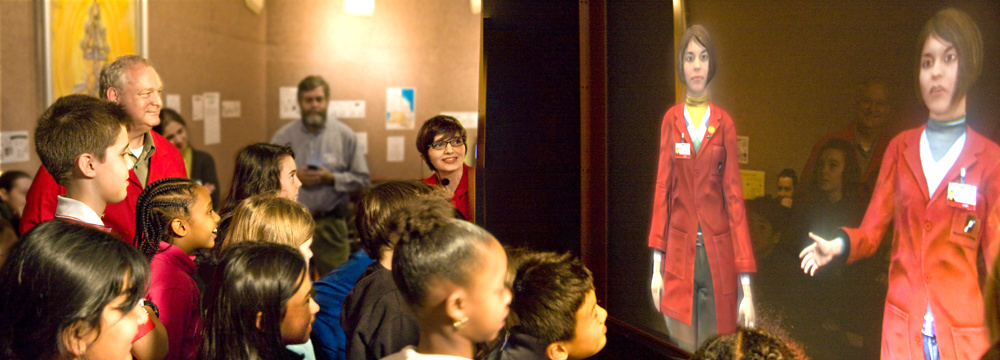
\includegraphics[width=0.9\textwidth,keepaspectratio=true]{images/ada_grace.jpg}
 \caption[Interaksi pemandu museum virtual Ada dan Grace dengan pengunjung di Museum of Science, Boston]{Interaksi pemandu museum virtual Ada dan Grace dengan pengunjung di Museum of Science, Boston \cite{armedwithscience-}.}
 \label{fig:ada_grace}
\vskip .5em
\end{figure}

Secara umum, implementasi ECA belum terlihat di Indonesia. Padahal, ECA dapat dimanfaatkan di berbagai bidang, misalnya di bidang pendidikan dan bidang pariwisata. ECA dapat dimanfaatkan sebagai tutor dalam proses pembelajaran. ECA juga dapat dimanfaatkan untuk membangun kios informasi pariwisata yang kemudian dapat ditempatkan di lokasi-lokasi yang mudah dijangkau oleh wisatawan, seperti di bandara, stasiun, terminal, hotel, atau bahkan di objek pariwisatanya sendiri. Implementasi ECA sebagai pemandu museum seperti Ada dan Grace dapat juga dilakukan di Indonesia untuk menarik lebih banyak orang untuk mengunjungi museum mengingat jumlah rata-rata pengunjung museum-museum di Indonesia pada kurun waktu 2006-2008 hanya mencapai 4,3 juta atau hanya 1,8 persen dari 237 juta lebih penduduk Indonesia (data tahun 2010) \cite{dppobappenas2009, bps2010}.

% RESTU's an Engine for Synthetic Thespian Units

Oleh karena itu, tim PUSPA dan SAMsON dari Program Magister Teknik Elektro, Sekolah Teknik Elektro dan Informatika (STEI), Institut Teknologi Bandung (ITB) bekerjasama dalam mengembangkan \textit{RESTU's an Engine for Synthetic Thespian Units} (RESTU), yang merupakan \textit{engine} untuk membangun ECA. Sebagai sebuah \textit{engine}, RESTU terdiri dari bagian interaksi dan bagian kognisi. Secara umum, bagian interaksi memanfaatkan monitor untuk menampilkan wujud agen, mikrofon sebagai telinga, kamera sebagai mata, dan speaker sebagai mulut. Sedangkan, bagian kognisi dapat dipilih untuk memanfaatkan AIML atau menggunakan \textit{artificial general intelligence} (AGI). Tim PUSPA sendiri memiliki tujuan membangun \textit{PUSPA’s an Understanding Synthespian that Provides Assistance} (PUSPA), yaitu sebuah ECA yang berperan sebagai asisten pribadi. Sedangkan, tim SAMsON memiliki tujuan membangun \textit{Smart Assistant for Museum's Objects Navigation} (SAMsON), yaitu sebuah ECA yang berperan sebagai pemandu museum \cite{nugraha2010}.

\begin{figure}[ht!]
\vskip 1em
\centering
 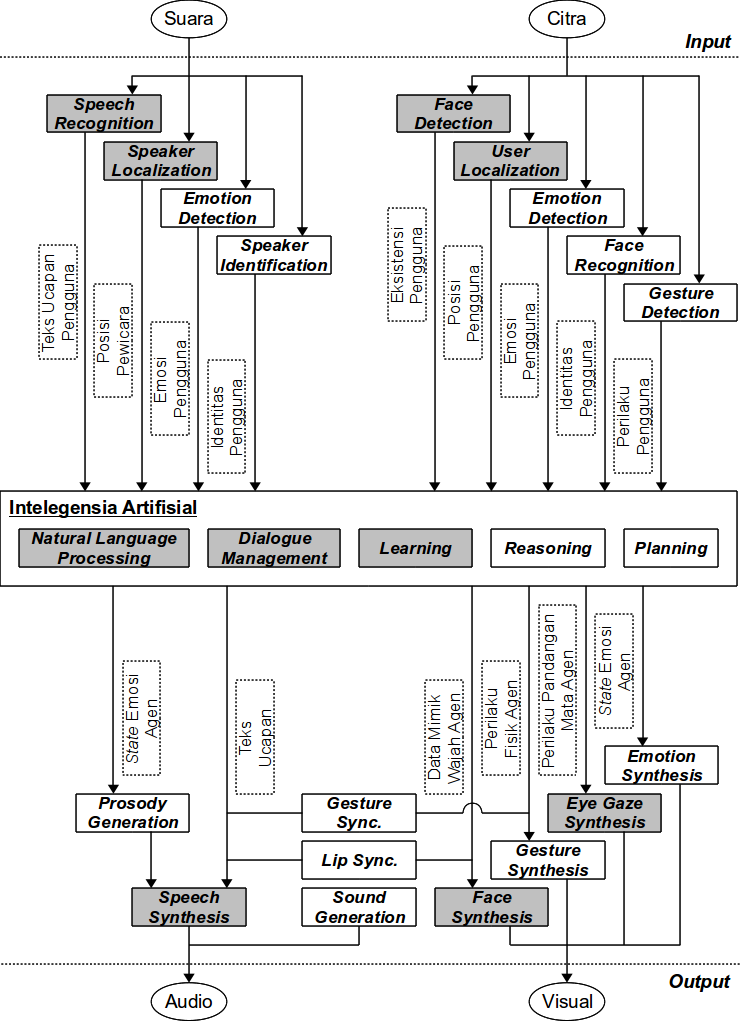
\includegraphics[width=\textwidth,keepaspectratio=true]{images/diagram_blok_eca.png}
 \caption[Diagram blok teknologi penyusun RESTU]{Diagram blok teknologi penyusun RESTU.}
 \label{fig:diagram_blok_eca}
\vskip .5em
\end{figure}

\autoref{fig:diagram_blok_eca} menunjukkan berbagai teknologi terkait ECA yang dapat diimplementasikan pada RESTU. Pada saat ini, teknologi yang diimplementasikan masih terbatas pada teknologi-teknologi yang dalam \autoref{fig:diagram_blok_eca} diberi \textit{background} berwarna abu-abu. Di luar teknologi-teknologi yang sudah tercantum, masih banyak teknologi yang berpotensi meningkatkan kemampuan interaksi ECA. Sebagai contoh, pada pengolahan masukan berupa suara (ucapan), terdapat teknologi \textit{speaker segmentation} dan \textit{speaker tracking}. Implementasi kedua teknologi ini pada RESTU akan memberi kemampuan pada ECA yang dihasilkan untuk mengelola komunikasi dengan pengguna lebih dari satu (\textit{multi-speaker environment}) \cite{martin2001}.

Seperti yang dapat dilihat pada \autoref{fig:diagram_blok_eca}, pada dasarnya komunikasi antara ECA dengan penggunanya hanya memanfaatkan media suara (audio) dan gambar (visual). Meskipun demikian, dari media audiovisual ini, berbagai komunikasi non-verbal dapat berlangsung, misalnya emosi pengguna dapat diketahui dari intonasi suaranya, ekspresi wajahnya, sikap tubuhnya, atau tatapan matanya. Di sisi lain, agen virtual juga dapat menunjukkan emosi yang beragam dengan memberi intonasi tertentu pada suara yang dihasilkan, ekspresi wajah tertentu, sikap tubuh serta pergerakan anggota badan tertentu, atau bahkan dengan tatapan mata tertentu \cite{morency2006, hartmann2005}.


% natural communication: face-to-face, implementation in ECA (need to know speaker location)

Dalam komunikasi tatap muka antar manusia, tatapan mata berperan penting dalam komunikasi non-verbal. Contoh yang paling sederhana adalah tatapan mata dapat memberi petunjuk kepada siapa seseorang sedang berbicara dan dapat memberi petunjuk kondisi emosi seseorang. Oleh karena ECA memiliki wujud, termasuk mata, tatapan mata sebagai salah satu metode komunikasi non-verbal ini juga dapat diimplementasikan untuk menciptakan komunikasi antara manusia dan komputer yang sama alaminya dengan komunikasi antar manusia. Implementasi tatapan mata dan pergerakan mata yang berbeda pada ECA juga telah terbukti memberikan kesan dan tingkat kepuasan yang berbeda bagi penggunanya \cite{lee2002, vanes2002}. Oleh karena itu, sebagai \textit{engine} ECA, RESTU juga harus mengakomodasi fitur ECA yang berupa tatapan dan pergerakan mata agen.

% source localization

Informasi yang dibutuhkan oleh agen dalam menentukan ke arah mana mata agen harus menatap adalah lokasi pengguna atau lawan bicara agen. Dalam RESTU, penentuan lokasi pengguna mungkin dilakukan dengan memanfaatkan informasi yang didapatkan dari: (1) sinyal suara yang ditangkap oleh mikrofon; dan/atau (2) citra yang ditangkap oleh kamera. Mempertimbangkan persyaratan \textit{modularity} dan \textit{extensibility} terkait modalitas masukan dan keluaran yang termasuk dalam persyaratan arsitektur ECA seperti yang tercantum dalam \cite{cassell1998}, penentuan lokasi pengguna dalam RESTU juga harus dapat dilakukan hanya berdasarkan sinyal suara saja atau gambar saja. Meskipun demikian, hasil penentuan lokasi kedua metode tersebut juga dapat dikombinasikan untuk memperoleh lokasi pengguna yang lebih akurat. Penentuan lokasi menggunakan citra yang ditangkap kamera cenderung menghasilkan nilai posisi yang lebih akurat. Akan tetapi, area dimana metode ini dapat digunakan lebih sempit dibandingkan area dimana metode penentuan lokasi menggunakan suara dapat digunakan. Analogi sederhananya adalah telinga manusia dapat mendengar suara yang berasal dari suatu posisi yang terletak di luar jangkauan pandangan mata, misalnya sebuah posisi yang terletak di belakang kepala.

\section{Tujuan Penelitian}

Secara umum, tujuan penelitian ini adalah merancang sebuah subsistem penentuan lokasi pengguna, yang merupakan komponen dari sistem ECA, berdasarkan sinyal suara yang ditangkap oleh mikrofon. Secara lebih khusus, penelitian ini bertujuan: (1) merancang subsistem penentuan lokasi pengguna untuk RESTU dengan memanfaatkan perangkat keras yang murah dan mudah didapatkan, serta perangkat lunak \textit{open source}; (2) mengimplementasikan rancangan yang dihasilkan pada RESTU; serta (3) mengujicoba subsistem penentuan lokasi pengguna yang telah diintegrasikan dalam RESTU.
\section{Batasan Masalah}
\label{sec:batasan}

Dalam perancangan subsistem penentuan lokasi pengguna berdasarkan sinyal suara ini, beberapa asumsi penting yang digunakan adalah sebagai berikut.

\begin{enumerate}
\item Hanya ada satu sumber suara yang dideteksi pada satu waktu.
\item Tidak ada derau dengan intensitas yang tinggi sedemikian sehingga suara ucapan yang tertangkap oleh mikrofon masih terdengar dengan jelas dan dominan.
\item Tidak ada efek akustik dari ruangan, misalnya gema atau gaung. Dengan kata lain, mikrofon hanya menangkap sinyal yang bersifat \textit{direct path} dari sumber suara.
\end{enumerate}

Subsistem penentuan lokasi pengguna yang dirancang memanfaatkan perangkat keras yang murah dan mudah didapatkan, serta perangkat lunak \textit{open source}. Perangkat keras utama yang dibutuhkan oleh subsistem ini adalah komputer, \textit{sound card}, dan mikrofon. Komputer yang digunakan memiliki prosesor Intel$^{\small{\textregistered}}$~Core\texttrademark~2 Duo T8100 2,1 GHz dan memori 2 GB. \textit{Sound card} yang digunakan adalah \textit{USB sound card} tanpa merk yang memiliki dua kanal keluaran (hanya mendukung \textit{sample rate} 48 KHz) dan satu kanal masukan (hanya mendukung \textit{sample rate} 24 KHz). Sedangkan, mikrofon yang digunakan adalah mikrofon \textit{omnidirectional} merk Genius. Subsistem dirancang dan diimplementasikan pada sistem operasi Ubuntu (Linux). Oleh karena kompatibilitas terhadap sistem operasi belum dipertimbangkan, subsistem tidak dapat dipastikan berjalan pada sistem operasi selain Ubuntu (Linux).

Subsistem penentuan lokasi pengguna yang dirancang akan diintegrasikan ke dalam RESTU. Sebagai \textit{showcase}, RESTU akan digunakan untuk membangun sebuah ECA yang berperan sebagai pemandu atau pusat informasi Laboratorium Sistem Komputer dan Kendali (LSKK), ITB. Perangkat keras yang akan digunakan untuk menampilkan pemandu virtual tersebut adalah perangkat \textit{multitouch screen} vertikal milik LSKK yang berdimensi 139 x 60 x 180 centimeter (panjang x lebar x tinggi) seperti yang terlihat pada \autoref{fig:multitouch-foto} dan \autoref{fig:multitouch-dim}. Layar berada di bagian atas dari salah satu sisi terluas perangkat. Pengguna diasumsikan manusia dewasa dengan tinggi badan 150-170 cm yang berdiri di depan layar pada jarak yang wajar diambil saat melakukan komunikasi tatap muka antar manusia (kurang lebih 1 meter). Pengguna juga diasumsikan menghadap ke layar saat berbicara, sedemikian sehingga sinyal suara yang dihasilkan dapat ditangkap oleh mikrofon-mikrofon yang ditempelkan pada perangkat.

\section{Sistematika Pembahasan}

BAB \ref{chap:pendahuluan} menguraikan sejarah singkat dan potensi-potensi pemanfaatan CA, serta proyek pengembangan RESTU, sebuah \textit{engine} ECA, yang kemudian menjadi latar belakang dan motivasi perancangan subsistem penentuan lokasi pengguna berdasarkan sinyal suara. \chaptername~ini juga mendefinisikan batasan-batasan yang digunakan dalam perancangan subsistem tersebut.

BAB \ref{chap:tinjauan_pustaka} membahas landasan teori terkait subsistem penentuan lokasi pengguna berdasarkan sinyal suara yang dirancang dalam penelitian ini. Pembahasan mencakup metode-metode penentuan lokasi sumber suara berdasarkan sinyal suara yang ditangkap.

%\autoref{chap:RESTU} menguraikan arsitektur RESTU secara umum dan menjelaskan bagaimana subsistem yang dirancang diintegrasikan di dalam RESTU.

BAB \ref{chap:perancangan} menjelaskan arsitektur RESTU secara umum dan hubungan subsistem yang dirancang dalam penelitian ini dengan subsistem-subsistem lain yang ada di dalam RESTU, serta menguraikan proses perancangan subsistem penentuan lokasi pengguna berdasarkan sinyal suara, yang meliputi perancangan perangkat keras dan lunak, proses pengambilan dan pengolahan data yang digunakan untuk melatih jaringan syaraf tiruan, serta proses pengujian dan analisis hasil pengujiannya.

BAB \ref{chap:integrasi} membahas proses integrasi subsistem penentuan lokasi pengguna berdasarkan sinyal suara ke dalam RESTU dan proses pengujiannya.

Sedangkan, BAB \ref{chap:kesimpulan} memuat kesimpulan dan saran berdasarkan penelitian yang dilakukan.
\subsection*{\textsf{\normalsize 2.2\hspace{0.5cm}KONSEP RANCANGAN}}
\addcontentsline{toc}{subsection}{2.2 KONSEP RANCANGAN}
\hyphenation{di-ba-ngun se-te-ngah}

\begin{figure}
	\centering
		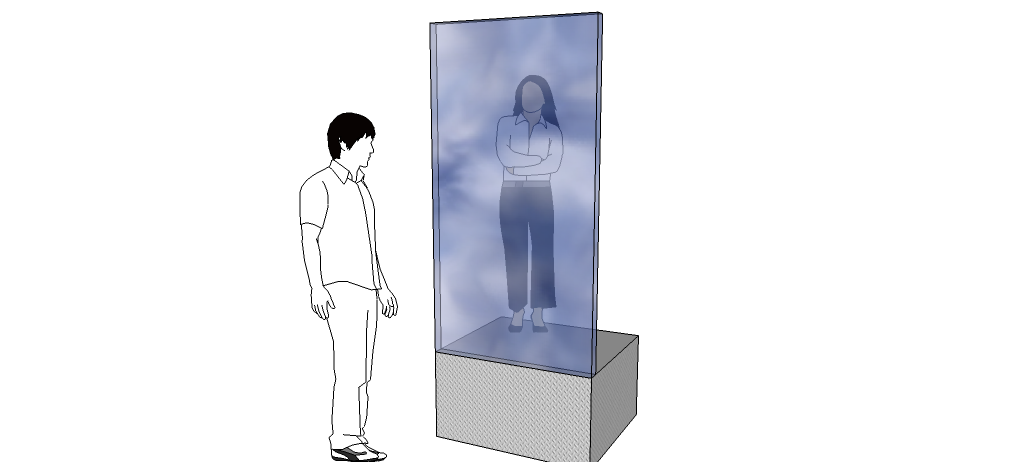
\includegraphics[scale=0.4]{konsep}
	\caption{Konsep instalasi PUSPA}
	\label{fig:konsep}
\end{figure}
Gambar~\ref{fig:konsep} menunjukkan ilustrasi instalasi PUSPA. Pada gambar tersebut terlihat seorang pengguna sedang berinteraksi dengan PUSPA melalui terminal \textit{holoscreen}. Di dalam terminal terlihat seorang asisten yang siap berinteraksi dengan pengguna. Asisten akan melirik ke kiri, kanan, bawah, maupun atas sesuai dengan posisi pengguna. Ia hanya akan diaktifkan jika pengguna adalah benar pemilik PUSPA, yang dapat dipastikan dengan mengenali wajahnya. Interaksi dengan PUSPA layaknya interaksi dengan manusia, yaitu komunikasi \textit{audiovisual}. Dia memiliki kepribadian, ekspresi, penglihatan dan pendengaran. Hal ini membuat seolah-olah PUSPA benar-benar hadir dalam kehidupan nyata. Inilah konsep dasar PUSPA.

PUSPA terdiri dari dua subsistem.
Subsistem pertama adalah subsistem \textit{server}, yang menjadi tempat pengolahan yang berhubungan dengan pembangkitan tanggapan.
Karena konsep PUSPA adalah \textit{client/server},
dimungkinkan agar PUSPA dapat berpindah-pindah terminal sesuai dengan posisi ruangan pengguna.
Subsistem ini menangani pada subsistem \textit{client} mana PUSPA harus ditampilkan.
Subsistem kedua adalah subsistem \textit{client}, yang berinteraksi dengan pengguna,
dan disebut juga sebagai terminal.

Sebagai sebuah \textit{synthespian},
PUSPA menampilkan rupa karakter dan segala pergerakannya.
Pada tahun 1988 Silicon Graphics dan deGraf-Wahrman Inc. bekerjasama dalam pembuatan animasi yang dikontrol oleh manusia.
Mereka merilis ``Mike The Talking Head'' yang menampilkan kepala yang dapat berbicara. \textit{Synthespian} dalam konsep rancangan PUSPA adalah model 3D kepala hingga setengah tubuh.
Adapun fitur \textit{synthespian} mencakup:
  \begin{itemize}
	\item \textit{photorealistic rendering},
	\item animasi emosi,
	\item animasi vokal,
	\item dan animasi panca indera (khususnya penglihatan).
  \end{itemize}
Daniel Thalmann, et al. dalam artikelnya \textit{Autonomous Virtual Actors Based on Virtual Sensors}, menuliskan bahwa \textit{synthespian} dapat memiliki panca indera melalui sensor.

PUSPA dilengkapi dengan antarmuka untuk interaksi selain yang dengan suara.
UI dalam PUSPA mengadopsi konsep \textit{soft control} dengan UI yang di-\textit{render} pada layar dengan desain yang menarik, dinamis, dan \textit{floating}.
Hal ini diperlukan karena \textit{input} pengguna menggunakan sensor sentuh.

Di samping semua itu,
PUSPA juga dilengkapi dengan \textit{multitouch holoscreen},
yang merupakan sebuah layar transparan dengan kemampuan \textit{touchscreen} multi-sentuh.
Contoh penerapan teknologi ini adalah pada produk Microsoft TouchLight.
Gambar~\ref{fig:tlight1} menunjukkan konfigurasi instalasi \textit{holoscreen},
dan Gambar~\ref{fig:tlight2} menggambarkan kemampuan multisentuh TouchLight.
Layar seperti inilah yang akan dikembangkan sebagai terminal PUSPA.
\begin{figure}
	\centering
		\subfloat[\textit{Holoscreen}]{\label{fig:tlight1}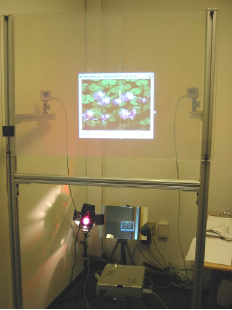
\includegraphics[scale=0.6]{tlight1}}\\
		\subfloat[\textit{Multitouch}]{\label{fig:tlight2}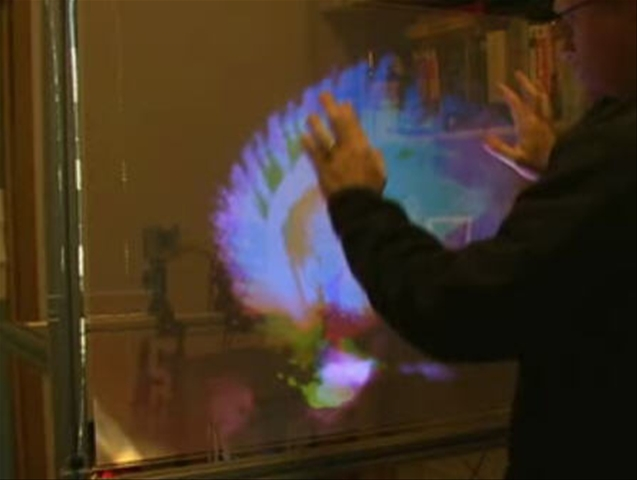
\includegraphics[scale=0.4]{tlight2}}
	\caption{Konfigurasi dan penggunaan touchlight}
	\label{fig:tlight}
\end{figure}	

\subsection*{\textsf{\normalsize 2.3\hspace{0.5cm}PERENCANAAN TEKNOLOGI}}
\addcontentsline{toc}{subsection}{2.3 PERENCANAAN TEKNOLOGI}
\hyphenation{ru-ang-an}

Teknologi yang diusung oleh PUSPA adalah
\begin{itemize}
	\item \textit{artificial intelligence};
	\item \textit{natural language processing};
	\item \textit{computer vision}, berupa akuisisi citra;
	\item \textit{surface computing};
	\item \textit{augmented reality},	dengan ditampilkannya PUSPA pada \textit{holoscreen};
	\item dan \textit{ubiquitous computing}, dengan dimungkinkannya PUSPA berpindah-pindah terminal sesuai dengan posisi ruangan pengguna.
\end{itemize}

\subsection*{\textsf{\normalsize 2.4\hspace{0.5cm}PERENCANAAN KERJASAMA}}
\addcontentsline{toc}{subsection}{2.4 PERENCANAAN KERJASAMA}

Kerjasama pengembang dan Laboratorium Sistem Kendali dan Komputer (LSKK) adalah pada pengembangan produk sebagai produk tesis program Beasiswa Unggulan Diknas, yang berarti pihak yang terlibat dalam pengembangan produk ini adalah:
\begin{enumerate}
	\item Tim Pengembang PUSPA, mahasiswa S2 program Teknologi Media Digital dan Game;
	\item LSKK, sebagai fasilitator dan tim ahli pengawas tim pengembang;
	\item dan Diknas, sebagai fasilitator beasiswa unggulan.
\end{enumerate}

Tim Pengembang PUSPA dan LSKK selanjutnya dapat bekerjasama dalam produksi dan pemasaran PUSPA, dan tentu saja masuknya investor sebagai pihak ketiga penyandang dana, misalnya seperti Lembaga Investasi RumahPemuda, dimungkinkan.
Harapannya adalah, dari pengembangan produk ini PUSPA dapat menghasilkan \textit{spin-off} berupa sebuah perusahaan yang mandiri.
 

\subsection*{\textsf{\normalsize 2.5\hspace{0.5cm}UPAYA PENGEMBANGAN}}
\addcontentsline{toc}{subsection}{2.5 UPAYA PENGEMBANGAN}
\hyphenation{de-ngan Speech-Recogniser}

Riset dan pengembangan PUSPA dilakukan oleh kelompok tesis yang saat ini anggotanya adalah:
\begin{itemize}
\item Erik Prabowo Kamal,
%\item Rio Andita Setiabakti,
\item dan Willy Derbyanto,
\end{itemize}
dengan kemungkinan penambahan anggota seiring dengan waktu dan kebutuhan, dan dengan pengawasan tim dan pembimbing tesis sebagai tim ahli.

Alat pengembangan yang digunakan adalah sebagai berikut:
\begin{itemize}
	\item Bahasa pemrograman: C++.
	\item Pustaka/\textit{Framework}: C++ Std Lib, Boost, OpenCog.
	\item \textit{Version control system}: Git.
	\item Dokumentasi: \LaTeX.
	\item Alat lainnya: CMake.
\end{itemize}

Pengembangan PUSPA dibagi menjadi tiga tahap:
\begin{itemize}
	\item Tahap I, tahap pengembangan fungsi dasar yang meliputi fungsi percakapan, dan fungsi yang berkaitan dengan rupa (\textit{modeling}, animasi dasar, dan \textit{rendering}).
	\item Tahap II, tahap pengembangan fungsi unggulan yang meliputi fungsi pelaksanaan tugas, mata dan kamera, kepribadian, animasi lanjut, dan pelacakan wajah pengguna.
	\item Tahap III, yaitu tahap pengembangan fungsi lanjut seperti hubungan \textit{client/server} fitur \textit{ubiquity}.
\end{itemize}
Ketiga tahapan tersebut dilaksanakan selama sembilan bulan. Tabel~\ref{tab:DevTime} menunjukkan tabel pembagian tugas dan waktu pengerjaannya.

\begin{table}
	\centering
		\begin{tabular}{|>{\small}l|>{\small}c|>{\small}p{4cm}|>{\small}c|>{\small}p{2cm}|}
		\hline
			\textbf{Proses\slash \textit{Task}} & 		\textbf{Tahap} & \textbf{\textit{Deliverables}} & \textbf{Jadwal} & \textbf{Kebutuhan Sumber Daya}\\
		\hline
			\multicolumn{5}{|>{\small}c|}{\textbf{\textit{Synthespian}}}\\
		\hline
			\textit{Modeling} & I & Model 3D kepala - torso lengkap dengan \textit{skeleton}-nya & 01/10/09 - 31/10/09 & 1 orang\\
		\hline
			Animasi dasar & I & Animasi-animasi dasar dari \textit{synthespian} & 02/11/09 - 28/11/09 & 1 orang\\
		\hline
			\textit{Real-time rendering} & I & Menampilkan \textit{synthespian} dalam \textit{engine} & 02/11/09 - 28/11/09 & 1 orang\\
		\hline
			Animasi kepribadian & II & Animasi berdasarkan sensor-sensor & 01/12/09 - 13/02/10 & 1 orang\\
		\hline
			Animasi vokal & II & Animasi vokal untuk berbicara & 16/02/10 - 30/04/10 & 1 orang\\
		\hline
			\multicolumn{5}{|>{\small}c|}{\textbf{Sensor dan Suara}}\\
		\hline
	Sensor penglihatan & II & Modul FaceDetector untuk mengenali wajah pengguna & 01/12/09 - 30/04/10 & 1 orang\\
		\hline
			Suara & II & Modul SpeechSynthesiser menyuarakan keluaran teks & 01/12/09 - 15/01/10 & 1 orang\\
		\hline
			Sensor pendengaran & II & Modul SpeechRecogniser mengenali perintah suara & 15/01/10 - 30/04/10 & 1 orang\\
		\hline
			\multicolumn{5}{|>{\small}c|}{\textbf{Antarmuka \textit{Soft Machine}}}\\
		\hline
			\textit{User Interface} & II & UI dengan \textit{soft control} & 01/02/10 - 27/02/10 & 1 orang\\
		\hline
			Layar & II & Layar multi-sentuh dengan 		\textit{holoscreen} & 01/03/10 - 30/04/10 & 1 orang\\
		\hline
			\multicolumn{5}{|>{\small}c|}{\textbf{\textit{Server}}}\\
		\hline
			\textit{Chatterbot} & I & Dapat menanggapi obrolan teks & 01/02/10 - 28/02/10 & 1 orang\\
		\hline
			Asisten & II & Dapat menanggapi tugas sebagai asisten: jadwal, tugas, dan \textit{to do} & 01/03/10 - 30/04/10 & 1 orang\\
		\hline
			\multicolumn{5}{|>{\small}c|}{\textbf{\textit{Client/Server}}}\\
		\hline
			\textit{Client-Server Dev.} & III & \textit{Client/server} untuk masing-masing terminal & 03/05/10 - 30/06/10 & 1 orang\\
		\hline
			\multicolumn{5}{|>{\small}c|}{\textbf{\textit{Finishing}}}\\
		\hline
			\textit{Bug fixing} & III & Pencarian \textit{bug} dan penyempurnaan produk & 03/05/10 - 30/06/10 & 1 orang\\
		\hline
	\end{tabular}
	\caption{Tugas dan jadwal pengembangan PUSPA}
	\label{tab:DevTime}
\end{table}

\subsection*{\textsf{\normalsize 2.6\hspace{0.5cm}UPAYA PRODUKSI}}
\addcontentsline{toc}{subsection}{2.6 UPAYA PRODUKSI}
\hyphenation{pe-ngem-bang-an}

Produksi PUSPA dapat dilaksanakan setelah purwarupa atau unit demonstrasi selesai dikembangkan. PUSPA tidak dikembangkan secara masal, namun menurut permintaan. Artinya PUSPA dipasarkan dengan unit demo di mana calon pengguna akan menyesuaikan PUSPA dengan kebutuhan pembeliannya. Oleh karena itu diperlukan tim produksi yang terpisah dengan tim riset dan pengembangan. Tim produksi memfokuskan diri pada kostumisasi PUSPA sesuai permintaan pembeli.

Kebutuhan bengkel utamanya adalah untuk aspek estetika terminal PUSPA, namun dapat pula produksi terminal khususnya integrasi layar dan CPU dialihdayakan ke pihak ketiga (\textit{outsourcing}). Hal ini dikarenakan investasi bengkel jauh lebih mahal ketimbang ongkos alih daya per unitnya, padahal yang dibutuhkan justru adalah komputer dan perangkat lunak pengembangan maupun produksi. 

PUSPA memiliki peluang keberhasilan di pasar, mengikuti analisis Gartner tahun 2009 tentang \textit{Hype Cycle of Emerging Technologies 2009} yang akan dijelaskan dalam analisis pasar, dengan \textit{market share} yang masih terbuka luas. Dengan asumsi penjualan sepuluh buah saja pada produksi tahun pertama, produk telah mencapai \textit{Break Event Point} (BEP).

Tabel~\ref{tab:ProdTime} menunjukkan ilustrasi mulai dari perencanaan dengan pembeli hingga \textit{delivery}.

\begin{table}
	\centering
		\begin{tabular}{|l|c|p{3.5cm}|c|p{3.5cm}|}
		\hline
			\textbf{Proses\slash \textit{Task}} & 		\textbf{Tahap} & \textbf{\textit{Deliverables}} & \textbf{Jadwal} & \textbf{Kebutuhan Sumber Daya}\\
		\hline
			\textit{Brainstorming} & I & Berita Acara Pertemuan desain PUSPA & 1-2 hari & 1 orang pemasaran\\
		\hline	
			Kesepakatan Kerjasama & I & MoU dengan pembeli & 1-2 hari & 1 orang pemasaran\\
		\hline
			Produksi PUSPA & II & Perangkat lunak siap di-\textit{install} ke terminal & 2 bulan & 3 orang pengembang\\
		\hline
			Produksi Terminal & II & Terminal yang siap di-\textit{deliver} & 2 minggu & 2 orang\\
		\hline
	\end{tabular}
	\caption{Ilustrasi jadwal produksi PUSPA}
	\label{tab:ProdTime}
\end{table}

\subsection*{\textsf{\normalsize 2.7\hspace{0.5cm}ESTIMASI BIAYA}}
\addcontentsline{toc}{subsection}{2.7 ESTIMASI BIAYA}

Lampiran A memperkirakan jumlah dana yang dibutuhkan untuk penelitian dan pengembangan PUSPA. Jumlah perkiraan investasinya adalah \textbf{Rp 68.150.000,00} yang semuanya dimanfaatkan untuk fasilitas awal.

Pada lampiran D, diperkirakan harga jual PUSPA adalah Rp 100.000.000,00 per unit. Dengan demikian batas biaya produksi adalah sepertiga harga jual, yaitu sebesar \textbf{Rp 33.000.000,00} per unit.

\subsection*{\textsf{\normalsize 2.8\hspace{0.5cm}ANALISIS PASAR}}
\addcontentsline{toc}{subsection}{2.8 ANALISIS PASAR}

Pengembangan PUSPA berpeluang menjadi perintis \textit{virtual personal assistant} maupun \textit{virtual friend}, di Indonesia. Teknologi yang diusung oleh PUSPA di antaranya adalah:
\begin{itemize}
	\item \textit{natural language processing},
	\item \textit{holoscreen} (\textit{surface computing}),
	\item \textit{augmented reality},
	\item dan \textit{ubiquitous computing},
\end{itemize}
yang paling tidak merupakan \textit{emerging technologies}.

Analisis yang dilakukan oleh lembaga riset \href{http://www.gartner.com}{Gartner} tentang ''\textit{Hype Cycle of Emerging Technologies}'' teknologi-teknologi di atas berada pada masa terobosan teknologi (\textit{technology trigger}). Gambar~\ref{fig:gartner} menunjukkan siklus Gartner yang dimaksud.

\begin{figure}
	\centering
		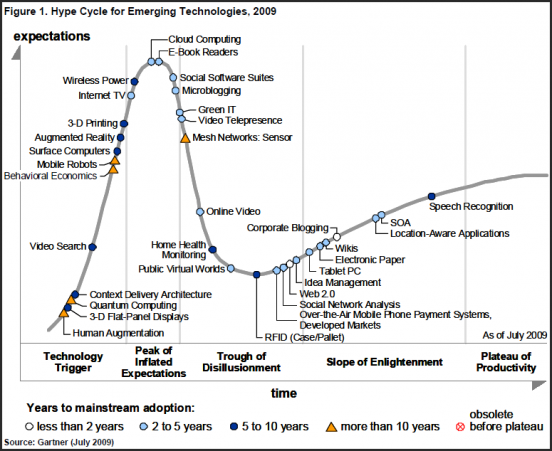
\includegraphics[scale=0.6]{gartner}
	\caption{Hype cycle of emerging technologies 2009 yang dipublikasikan oleh Gartner}
	\label{fig:gartner}
\end{figure}

Pada masa terobosan teknologi, pasar belum terpetakan dan \textit{market share} pun belum dibatasi. Sistem pemasarannya pun masih melalui pembahasan di media, demonstrasi publik di pameran-pameran, dan sebagainya. Kondisi ini adalah peluang besar untuk masuk ke pasar dan melakukan \textit{branding}.

Saat ini produk sejenis yang dapat berpeluang menjadi pesaing adalah produk Site Pal, dengan \textit{chatterbot} \href{http://alice.pandorabots.com}{A.L.I.C.E.}. Namun Site Pal adalah produk berbasis \textit{web}, sedangkan PUSPA berbentuk terminal.
Bagaimanapun, antarmuka \textit{web} untuk peran \textit{chatterbot} (tapi tidak untuk peran asisten) tetap dibuat untuk keperluan publikasi dan promosi.

Memasuki pasar pada masa terobosan teknologi memiliki kelemahan yaitu investasi pendidikan produk \textit{product knowledge} kepada masyarakat untuk memperbanyak pasar, sehingga target pasar PUSPA masih terbatas pada:
\begin{enumerate}
	\item museum,
	\item \textit{tenant} dan manajemen mal,
	\item perkantoran,
	\item dan aplikator rumah pintar,
\end{enumerate}
di mana kehadiran PUSPA secara umum diperlukan. Dengan target penjualan yang tidak terlalu tinggi, sepuluh saja per tahun, sudah dapat menghasilkan pendapatan usaha yang signifikan.


\subsection*{\textsf{\normalsize 2.9\hspace{0.5cm}UPAYA PEMASARAN}}
\addcontentsline{toc}{subsection}{2.9 UPAYA PEMASARAN}
\hyphenation{me-ngem-bang-kan mem-ben-tang-kan}

Dikarenakan produk PUSPA masih berada dalam masa terobosan teknologi, langkah pemasaran yang cocok adalah:
\begin{enumerate}
	\item pembahasan teknologi,
	\item \textit{launching} produk pada \textit{event}-\textit{event} tertentu, dan
	\item demonstrasi di depan publik.
\end{enumerate}
Ketiga langkah di atas bertujuan untuk menarik perhatian media massa dan industri, sehingga mereka tertarik untuk membeli. Ketiganya dapat dilakukan dalam satu \textit{event}, yaitu pameran.

Pemasaran PUSPA harus dilakukan melalui pameran-pameran teknologi. Berikut ini adalah strategi yang setidaknya harus dilakukan untuk memasarkan PUSPA di Indonesia.
\begin{itemize}
	\item Mengikutsertakan PUSPA dalam lomba-lomba teknologi dan bisnis, misalnya INAICTA.
	\item Mengikutsertakan PUSPA dalam pameran-pameran yang diadakan oleh ITB, misalnya Digital Media dan Game Festival.
	\item Mengikutsertakan PUSPA dalam pameran-pameran Departemen Kominfo dan Ristek, misalnya pameran RISTI.
	\item Mengikutsertakan PUSPA dalam pameran-pameran industri, misalnya FGDExpo.
\end{itemize}
Semua pameran tersebut di atas dilaksanakan setiap tahun di Indonesia.

Selain keikutsertaan dalam berbagai pameran, tim pemasaran PUSPA pun mengembangkan jaringan bisnis dengan menjadi anggota komunitas tertentu misalnya Bandung High Tech Valley, Bandung Creative City, dan lain sebagainya. Hal ini diperlukan untuk membentangkan jaringan bisnis dan pengetahuan akan perusahaan pengembang PUSPA. Tim pemasaran pun perlu mengikuti aktivitas inkubasi-inkubasi bisnis yang mulai marak dan tumbuh kembang di Indonesia.

\subsection*{\textsf{\normalsize 2.10\hspace{0.5cm}PERHITUNGAN \textit{NET PRESENT VALUE} (NPV)}}
\addcontentsline{toc}{subsection}{2.10 PERHITUNGAN \textit{NET PRESENT VALUE}}

Dalam Lampiran C hingga F dilampirkan perhitungan aliran kas (\textit{cashflow}). Dari data pada Lampiran F didapat \textit{Net Cash Flow} per tahun. Dengan asumsi \textit{discount rate} sebesar 15\% didapatkan NPV dengan perhitungan seperti pada Tabel~\ref{tab:npv}.

Nilai NPV yang didapat adalah sebesar Rp 4.137.265.900. Dengan NPV $>$ 0, dapat disimpulkan bahwa pengembangan PUSPA adalah layak usaha.

\begin{table}
	\centering
		\begin{tabular}{|>{\scriptsize}p{1.4cm}|>{\scriptsize}r|>{\scriptsize}r|>{\scriptsize}r|>{\scriptsize}r|>{\scriptsize}r|>{\scriptsize}r|}
\hline
\textbf{Tahun Ke-} & \textbf{0} & \textbf{1} & \textbf{2} & \textbf{3} & \textbf{4} & \textbf{5}\\
\hline
\multicolumn{7}{c}{}\\
\hline
\textbf{Interest Rate} & 15,00\% & \multicolumn{5}{c|}{}\\
\hline
\textbf{Discounted Factor} & 1,00 & 0,87 & 0,76 & 0,66 & 0,57 & 0,50\\
\hline
\textbf{NCF} & Rp100.000.000 & Rp311.850.000 & Rp855.720.000 & Rp1.384.092.000 & Rp1.847.092.000 & Rp2.720.092.000\\
\hline
\textbf{PV} & Rp100.000.000 & Rp271.173.913 & Rp647.047.259 & Rp910.062.957 & Rp1.056.366.723 & Rp1.352.615.049\\
\hline
\textbf{NPV} & Rp4.137.265.900 & \multicolumn{5}{c|}{}\\
\hline
\end{tabular}

	\caption{Tabel perhitungan NPV}
	\label{tab:npv}
\end{table}

\subsection*{\textsf{\normalsize 2.11\hspace{0.5cm}DAFTAR \textit{DELIVERABLES}, SPESIFIKASI, DAN JADWALNYA}}
\addcontentsline{toc}{subsection}{2.11 DAFTAR \textit{DELIVERABLES}, SPESIFIKASI, DAN JADWALNYA}
\hyphenation{ke-ya-kin-an}

\textit{Deliverables} pengembangan PUSPA disesuaikan dengan tahapan pengembangan, yaitu:
\begin{enumerate}
	\item Tahap I\\
	Tanggal \textit{release}: 1 Maret 2010\\
	PUSPA dengan fungsi dasar yaitu \textit{chatterbot} dengan \textit{synthespian} yang masih sederhana.
	\item Tahap II\\
	Tanggal \textit{release}: 1 Mei 2010\\
	PUSPA dengan peran asisten dan fungsi lengkap \textit{client}.
	\item Tahap II\\
	Tanggal \textit{release}: 1 Juli 2010\\
	PUSPA dengan fungsi lengkap \textit{client-server}.
\end{enumerate}

\subsection*{\textsf{\normalsize 2.12\hspace{0.5cm}KESIMPULAN}}
\addcontentsline{toc}{subsection}{2.12 KESIMPULAN}
\hyphenation{Pro-ses}

Dapat disimpulkan bahwa riset dan pengembangan PUSPA memiliki potensi keuntungan yang sangat besar dengan modal awal yang sangat kecil. Tentu saja proses riset dan pengembangan yang terlalu singkat dan bercampur dengan penulisan tesis menjadi tantangan tersendiri. Proses produksi dan pemasaran yang masih mengambang di benak kami turut melemahkan posisi tawar dokumen ini. Namun kami yakin, riset dan pengembangan PUSPA akan memberikan hasil yang positif baik dari segi bisnis maupun riset internal di lingkungan LSKK, STEI--ITB. Ditambah dengan nilai NPV sebesar Rp 4.137.265.900 keyakinan kami semakin tajam. Kami tentunya berharap realisasi dari dokumen ini agar segera dijalankan, mengingat keterbatasan waktu pengembangan.



\appendix
\addcontentsline{toc}{section}{LAMPIRAN}

\section{Diagram Gantt Pengembangan PUSPA}
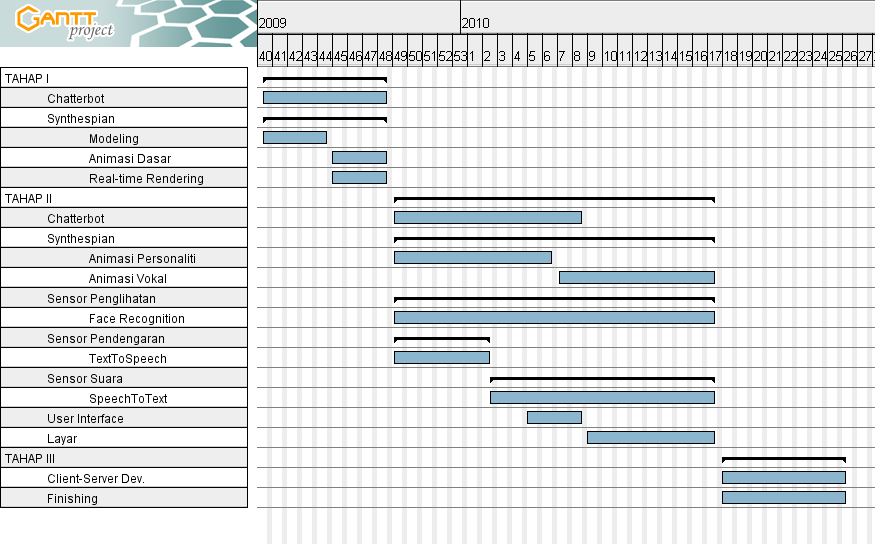
\includegraphics[scale=0.5]{gant}

\section{Beban Kerja Pengembangan PUSPA}
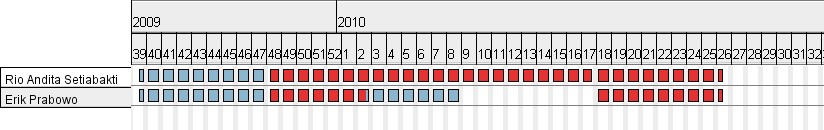
\includegraphics[scale=0.5]{manhour}
\section{Rencana Anggaran Awal}
\begin{tabular}{|>{\small}c|>{\small}p{4cm}|>{\small}r|>{\small}c|>{\small}c|>{\small}r|}
\hline
No. & Keterangan & Harga Satuan (Rp) & Jumlah & Satuan & Total Harga (Rp)\\
\hline
\multicolumn{2}{|>{\small}l|}{FASILITAS PRODUKSI} & & & & \\
\hline
1 & Komputer Desain & 5.000.000 & 1 & Set & 5.000.000\\
\hline
2 & Komputer Programming & 5.000.000 & 1 & Set & 5.000.000\\
\hline
3 & WACOM Sketch Tablet & 2.000.000 & 1 & Unit & 2.000.000\\
\hline
4 & Recording Tools & 5.000.000 & 1 & Unit & 5.000.000\\
\hline
\multicolumn{2}{|>{\small}l|}{DEMO UNIT} & & & & \\
\hline
\multicolumn{2}{|>{\small}l|}{MULTITOUCH UNIT} & & 2 & & \\
\hline
1 & Rear Projection Film & 10.000.000 & 1 & Roll & 10.000.000\\
\hline
2 & FFMV-03M2M-CS & 2.950.000 & 2 & Unit & 5.900.000\\
\hline
3 & DEVKIT-01-0005 & 550.000 & 1 & Unit & 550.000\\
\hline
4 & YV5x2.7R4B-2 & 650.000 & 2 & Unit & 1.300.000\\
\hline
5 & Customised BP800 filter, slipmount, CA30 & 1.650.000 & 2 & Unit & 3.300.000\\
\hline
6 & Akrilik (16:9) 42" & 500.000 & 2 & Unit & 1.000.000\\
\hline
7 & Proyektor & 6.000.000 & 2 & Unit & 12.000.000\\
\hline
\multicolumn{2}{|>{\small}l|}{TERMINAL UNIT} & & 2 & & \\
\hline
1 & Komputer & 0 & 2 & Lump Sum & 0\\
\hline
 & & & & & \\
\hline
\multicolumn{2}{|>{\small}l|}{SERVER NETWORKING UNIT} & & 2 & &\\
\hline
1 & Server & 3.500.000 & 1 & Unit & 3.500.000\\
\hline
2 & WiFi Router & 1.000.000 & 1 & Unit & 1.000.000\\
\hline
3 & USB WiFi & 300.000 & 2 & Unit & 600.000\\
\hline
 & & & & & \\
\hline
\multicolumn{2}{|>{\small}l|}{LAIN-LAIN} & & 2 & & \\
\hline
1 & Booth Kit & 2.000.000 & 1 & Lump Sum & 2.000.000\\
\hline
2 & Registrasi HKI & 10.000.000 & 1 & Lump Sum & 10.000.000\\
\hline
3 & Lain-lain & 0 & 1 & Lump Sum & 0\\
\hline
\multicolumn{2}{|>{\small}l|}{BIAYA TOTAL} & & & & 68.150.000\\
\hline
\end{tabular}

\section{Rancangan Gaji (\textit{Manhour Rate})}

\begin{tabular}{|>{\scriptsize}p{0.5cm}|>{\scriptsize}p{2.3cm}|>{\scriptsize\raggedleft}p{0.8cm}|>{\scriptsize\centering}p{1cm}|>{\scriptsize\raggedleft}p{0.9cm}|>{\scriptsize\raggedleft}p{0.8cm}|>{\scriptsize\centering}p{1cm}|>{\scriptsize\raggedleft}p{1cm}|>{\scriptsize\raggedleft}p{0.8cm}|>{\scriptsize\centering}p{1cm}|>{\scriptsize\raggedleft}p{1cm}|p{0pt}}
\cline{1-11}
\multirow{2}{*}{No.} & \multirow{2}{*}{Posisi} & \multicolumn{3}{>{\scriptsize}c|}{TAHUN I} & \multicolumn{3}{>{\scriptsize}c|}{TAHUN II} & \multicolumn{3}{>{\scriptsize}c|}{TAHUN III-V} & \\
\cline{3-11}
 & & \raggedright Gaji per Bulan (Rp 1.000) & \raggedright Banyak Personil (orang) & \raggedright Total Gaji per Tahun (Rp 1.000) & \raggedright Gaji per Bulan (Rp 1.000) & \raggedright Banyak Personil (orang) & \raggedright Total Gaji per Tahun (Rp 1.000) & \raggedright Gaji per Bulan (Rp 1.000) & \raggedright Banyak Personil (orang) & \raggedright Total Gaji per Tahun (Rp 1.000) & \\
\cline{1-11}
A & MANAJEMEN & & & & & & & & & & \\
\cline{1-11}
1 & CEO (sekaligus COO) & 5.000 & 0,5 & 32.500 & 5.500 & 1 & 71.500 & 6.050 & 1 & 78.650 & \\
\cline{1-11}
2 & CTO & 4.000 & 0,5 & 26.000 & 4.400 & 1 & 57.200 & 4.840 & 1 & 62.920 & \\
\cline{1-11}
 & & & & & & & & & & & \\
\cline{1-11}
B & PRODUKSI, R\&D & & & & & & & & & & \\
\cline{1-11}
1 & Development Manager & 3.500 & 0 & 0 & 3.850 & 1 & 50.050 & 4.235 & 1 & 55.055 & \\
\cline{1-11}
2 & Programmer & 2.000 & 0 & 0 & 2.200 & 2 & 57.200 & 2.420 & 2 & 62.920 & \\
\cline{1-11}
3 & Artist & 2.000 & 0 & 0 & 2.200 & 2 & 57.200 & 2.420 & 2 & 62.920 & \\
\cline{1-11}
4 & Content Designer & 2.000 & 0 & 0 & 2.200 & 1 & 28.600 & 2.420 & 1 & 31.460 & \\
\cline{1-11}
 & & & & & & & & & & & \\
\cline{1-11}
C & OPERASIONAL & & & & & & & & & & \\
\cline{1-11}
1 & Marketing Manager & 3.500 & 0 & 0 & 3.850 & 1 & 50.050 & 4.235 & 1 & 55.055 & \\
\cline{1-11}
2 & Marketing Staff & 2.000 & 0 & 0 & 2.200 & 3 & 85.800 & 2.420 & 3 & 94.380 & \\
\cline{1-11}
3 & Administration Staff & 2.000 & 0 & 0 & 2.200 & 1 & 28.600 & 2.420 & 1 & 31.460 & \\
\cline{1-11}
4 & Customer Service & 1.500 & 0 & 0 & 1.650 & 6 & 128.700 & 1.815 & 6 & 141.570 & \\
\cline{1-11}
5 & General Function Staff & 1.000 & 0 & 0 & 1.100 & 1 & 14.300 & 1.210 & 1 & 15.730 & \\
\cline{1-11}
 & & & & & & & & & & & \\
\cline{1-11}
\multicolumn{4}{|>{\scriptsize}l|}{JUMLAH GAJI} & 58.500 & \multicolumn{2}{c|}{} & 629.200 & \multicolumn{2}{c|}{} & 692.120 & \\
\cline{1-11}
\end{tabular}

\section{Proyeksi Laba Rugi}
\raggedright
\begin{tabular}{|>{\tiny}c|>{\tiny}p{2.3cm}|>{\tiny}c|>{\tiny}c|>{\tiny\raggedleft}p{1.2cm}|>{\tiny}c|>{\tiny}c|>{\tiny\raggedleft}p{1.2cm}|>{\tiny}c|>{\tiny}c|>{\tiny\raggedleft}p{1.2cm}|p{0pt}}
\cline{1-11}
\multirow{2}{*}{No.} & \centering \multirow{2}{*}{Deskripsi} & \multicolumn{3}{>{\tiny}c|}{TAHUN I} & \multicolumn{3}{>{\tiny}c|}{TAHUN II} & \multicolumn{3}{>{\tiny}c|}{TAHUN III} & \\
\cline{3-11}
 & & Byk. & Satuan & \centering Nilai (Rp 1.000) & Byk. & Satuan & \centering Nilai (Rp 1.000) & Byk. & Satuan & \centering Nilai (Rp 1.000) & \\
\cline{1-11}
 & PEMASUKAN & & & & & & & & & & \\
\cline{1-11}
1 & Penjualan PUSPA & 10 & Unit & 1.000.000 & 20 & Unit & 2.000.000 & 10 & Unit & 1.000.000 & \\
\cline{1-11}
2 & Penjualan Produk Baru Thn. II & 0 & & 0 & 10 & Unit & 1.000.000 & 20 & Unit & 2.000.000 & \\
\cline{1-11}
3 & Penjualan Produk Baru Thn. III & 0 & & 0 & 0 & & 0 & 10 & Unit & 1.000.000 & \\
\cline{1-11}
4 & Penjualan Produk Baru Thn. IV & 0 & & 0 & 0 & & 0 & 0 & & 0 & \\
\cline{1-11}
5 & Penjualan Produk Baru Thn. V & 0 & & 0 & 0 & & 0 & 0 & & 0 & \\
\cline{1-11}
6 & Distributor Fee & 0 & Distributor & 0 & 0 & Dist & 0 & 0 & Dist & 0 & \\
\cline{1-11}
 & Total Pemasukan & & & 1.000.000 & & & 3.000.000 & & & 4.000.000 & \\
\cline{1-11}
 & PENGELUARAN & & & & & & & & & & \\
\cline{1-11}
1 & Gaji & 1 & Lump Sum & 58.500 & 1 & Lump Sum & 629.200 & 1 & Lump Sum & 692.120 & \\
\cline{1-11}
2 & Modal Produksi & 10 & Unit & 330.000 & 30 & Unit & 990.000 & 40 & Unit & 1.320.000 & \\
\cline{1-11}
3 & Biaya Maintenance \& Service & 1 & Lump Sum & 30.000 & 1 & Lump Sum & 60.000 & 1 & Lump Sum & 60.000 & \\
\cline{1-11}
4 & Biaya Operasional & 1 & Lump Sum & 30.000 & 1 & Lump Sum & 60.000 & 1 & Lump Sum & 60.000 & \\
\cline{1-11}
5 & Biaya Administrasi & 1 & Lump Sum & 30.000 & 1 & Lump Sum & 60.000 & 1 & Lump Sum & 60.000 & \\
\cline{1-11}
6 & Biaya Pengembangan Produk & 1 & Lump Sum & 100.000 & 1 & Lump Sum & 100.000 & 1 & Lump Sum & 120.000 & \\
\cline{1-11}
7 & Listrik \& Air & 1 & Lump Sum & 30.000 & 1 & Lump Sum & 60.000 & 1 & Lump Sum & 60.000 & \\
\cline{1-11}
8 & Telepon \& Internet & 1 & Lump Sum & 30.000 & 1 & Lump Sum & 60.000 & 1 & Lump Sum & 60.000 & \\
\cline{1-11}
9 & Lain-lain & 1 & Lump Sum & 15.000 & 1 & Lump Sum & 30.000 & 1 & Lump Sum & 30.000 & \\
\cline{1-11}
 & Total Pengeluaran & & & 653.500 & & & 2.049.200 & & & 2.462.120 & \\
\cline{1-11}
 & Laba - Rugi & & & 346.500 & & & 950.800 & & & 1.537.880 & \\
\cline{1-11}
\end{tabular}

\begin{tabular}{|>{\tiny}c|>{\tiny}p{2.3cm}|>{\tiny}c|>{\tiny}c|>{\tiny\raggedleft}p{1.2cm}|>{\tiny}c|>{\tiny}c|>{\tiny\raggedleft}p{1.2cm}|p{0pt}}
\cline{1-8}
\multirow{2}{*}{No.} & \centering \multirow{2}{*}{Deskripsi} & \multicolumn{3}{>{\tiny}c|}{TAHUN IV} & \multicolumn{3}{>{\tiny}c|}{TAHUN V} & \\
\cline{3-8}
 & & Byk. & Satuan & \centering Nilai (Rp 1.000) & Byk. & Satuan & \centering Nilai (Rp 1.000) & \\
\cline{1-8}
 & PEMASUKAN & & & & & & & \\
\cline{1-8}
1 & Penjualan PUSPA & 5 & Unit & 500.000 & 5 & Unit & 500.000 & \\
\cline{1-8}
2 & Penjualan Produk Baru Thn. II & 10 & Unit & 1.000.000 & 10 & Unit & 1.000.000 & \\
\cline{1-8}
3 & Penjualan Produk Baru Thn. III & 20 & Unit & 2.000.000 & 10 & Unit & 1.000.000 & \\
\cline{1-8}
4 & Penjualan Produk Baru Thn. IV & 10 & Unit & 1.000.000 & 20 & Unit & 2.000.000 & \\
\cline{1-8}
5 & Penjualan Produk Baru Thn. V & 0 & & 0 & 10 & Unit & 1.000.000 & \\
\cline{1-8}
6 & Distributor Fee & 2 & Dist & 300.000 & 4 & Dist & 600.000 & \\
\cline{1-8}
 & Total Pemasukan & & & 4.800.000 & & & 6.100.000 & \\
\cline{1-8}
 & PENGELUARAN & & & & & & & \\
\cline{1-8}
1 & Gaji & 1 & Lump Sum & 692.120 & 1 & Lump Sum & 692.120 & \\
\cline{1-8}
2 & Modal Produksi & 45 & Unit & 1.485.000 & 55 & Unit & 1.815.000 & \\
\cline{1-8}
3 & Biaya Maintenance \& Service & 1 & Lump Sum & 120.000 & 1 & Lump Sum & 120.000 & \\
\cline{1-8}
4 & Biaya Operasional & 1 & Lump Sum & 120.000 & 1 & Lump Sum & 120.000 & \\
\cline{1-8}
5 & Biaya Administrasi & 1 & Lump Sum & 60.000 & 1 & Lump Sum & 60.000 & \\
\cline{1-8}
6 & Biaya Pengembangan Produk & 1 & Lump Sum & 120.000 & 1 & Lump Sum & 120.000 & \\
\cline{1-8}
7 & Listrik \& Air & 1 & Lump Sum & 60.000 & 1 & Lump Sum & 60.000 & \\
\cline{1-8}
8 & Telepon \& Internet & 1 & Lump Sum & 60.000 & 1 & Lump Sum & 60.000 & \\
\cline{1-8}
9 & Lain-lain & 1 & Lump Sum & 30.000 & 1 & Lump Sum & 30.000 & \\
\cline{1-8}
 & Total Pengeluaran & & & 2.747.120 & & & 3.077.120 & \\
\cline{1-8}
 & Laba - Rugi & & & 2.052.880 & & & 3.022.880 & \\
\cline{1-8}
\end{tabular}
\section{Perkiraan \textit{Cashflow} per Tahun}
\begin{tabular}{|>{\scriptsize}p{2.5cm}|>{\scriptsize}r|>{\scriptsize}r|>{\scriptsize}r|>{\scriptsize}r|>{\scriptsize}r|>{\scriptsize}r|}
\hline
 & & TAHUN I & TAHUN II & TAHUN III & TAHUN IV & TAHUN V\\
\hline
CASH INFLOW & & & & & & \\
\hline
Modal & 100.000.000 & & & & & \\
\hline
Penjualan PUSPA & & 1.000.000.000 & 2.000.000.000 & 1.000.000.000 & 500.000.000 & 500.000.000\\
\hline
Penjualan Produk Baru Thn II & & 0 & 1.000.000.000 & 2.000.000.000 & 1.000.000.000 & 1.000.000.000\\
\hline
Penjualan Produk Baru Thn III & & 0 & 0 & 1.000.000.000 & 2.000.000.000 & 1.000.000.000\\
\hline
Penjualan Produk Baru Thn IV & & 0 & 0 & 0 & 1.000.000.000 & 2.000.000.000\\
\hline
Penjualan Produk Baru Thn V & & 0 & 0 & 0 & 0 & 1.000.000.000\\
\hline
Distributor Fee & & 0 & 0 & 0 & 300.000.000 & 600.000.000\\
\hline
Total Cash Inflow & 100.000.000 & 1.000.000.000 & 3.000.000.000 & 4.000.000.000 & 4.800.000.000 & 6.100.000.000\\
\hline
 & & & & & & \\
\hline
CASH OUTFLOW & & & & & & \\
\hline
Fasilitas Awal & 68.150.000 & & & & & \\
\hline
Modal Produksi & & 330.000.000 & 990.000.000 & 1.320.000.000 & 1.485.000.000 & 1.815.000.000\\
\hline
Beban Gaji & & 58.500.000 & 629.200.000 & 692.120.000 & 692.120.000 & 692.120.000\\
\hline
Biaya-biaya & & 265.000.000 & 430.000.000 & 450.000.000 & 570.000.000 & 570.000.000\\
\hline
Sewa Kantor & & 0 & 120.000.000 & 120.000.000 & 120.000.000 & 120.000.000\\
\hline
Total Cash Outflow & 68.150.000 & 653.500.000 &2.049.200.000 & 2.462.120.000 & 2.747.120.000 & 3.077.120.000\\
\hline
 & & & & & & \\
\hline
Net Cash Flow & 31.850.000 & 346.500.000 & 950.800.000 & 1.537.880.000 & 2.052.880.000 & 3.022.880.000\\
\hline
Net Cash Flow Setelah Pajak & 31.850.000 & 311.850.000 & 855.720.000 & 1.384.092.000 & 1.847.592.000 & 2.720.592.000\\
\hline
Cumulative Net Cash Flow & 31.850.000 & 343.700.000 & 1.199.420.000 & 2.583.512.000 & 4.431.104.000 & 7.151.696.000\\
\hline
 & & & & & & \\
\hline
\end{tabular}

\begin{tabular}{|>{\scriptsize}p{1.4cm}|>{\scriptsize}r|>{\scriptsize}r|>{\scriptsize}r|>{\scriptsize}r|>{\scriptsize}r|>{\scriptsize}r|}
\multicolumn{7}{c}{}\\
\multicolumn{7}{c}{\textbf{ANALISIS KELAYAKAN USAHA}}\\
\hline
\textbf{Tahun Ke-} & \textbf{0} & \textbf{1} & \textbf{2} & \textbf{3} & \textbf{4} & \textbf{5}\\
\hline
\multicolumn{7}{c}{}\\
\hline
\textbf{Interest Rate} & 15,00\% & \multicolumn{5}{c|}{}\\
\hline
\textbf{Discounted Factor} & 1,00 & 0,87 & 0,76 & 0,66 & 0,57 & 0,50\\
\hline
\textbf{NCF} & Rp100.000.000 & Rp311.850.000 & Rp855.720.000 & Rp1.384.092.000 & Rp1.847.092.000 & Rp2.720.092.000\\
\hline
\textbf{PV} & Rp100.000.000 & Rp271.173.913 & Rp647.047.259 & Rp910.062.957 & Rp1.056.366.723 & Rp1.352.615.049\\
\hline
\textbf{NPV} & Rp4.137.265.900 & \multicolumn{5}{c|}{}\\
\hline
\multicolumn{7}{c}{}\\
\hline
\textbf{Interest Rate} & 16,00\% & \multicolumn{5}{c|}{}\\
\hline
\textbf{Discounted Factor} & 1,00 & 0,86 & 0,74 & 0,64 & 0,55 & 0,48\\
\hline
\textbf{NCF} & Rp100.000.000 & Rp311.850.000 & Rp855.720.000 & Rp1.384.092.000 & Rp1.847.592.000 & Rp2.720.592.000\\
\hline
\textbf{PV} & Rp100.000.000 & Rp268.836.207 & Rp635.939.358 & Rp886.729.161 & Rp1.020.408.614 & Rp1.295.309.261\\
\hline
\textbf{NPV} & Rp4.007.222.600 & \multicolumn{5}{c|}{}\\
\hline
\multicolumn{7}{c}{}\\
\hline
IRR & 46,81\% & \multicolumn{5}{c|}{}\\
\hline
\end{tabular}

\section{Biodata Pengusul}

\subsection*{Pengusul 1}

\subsubsection*{Data Pribadi}
\begin{tabular}{ll}
Nama & : Erik Prabowo Kamal\\
Tempat\slash tanggal lahir & : Jakarta, 6 Mei 1979\\
Alamat & : Jln. Ligar Kencana Blok B No. 8 Bandung 40191, Indonesia\\
Nomor telepon & : +62818194507, +62222509262\\
Alamat \textit{e-mail} & : \href{mailto:erik@rumahtenda.web.id}{erik@rumahtenda.web.id}
\end{tabular}

\subsubsection*{Keahlian}
\begin{tabular}{ll}
Alat pengembangan perangkat lunak & : Apple Xcode, GNU toolchain, GNU Emacs\\
Alat pengembangan perangkat keras & : gEDA suite\\
Bahasa pemrograman & : C, C++, Objective-C\\
Pustaka & : C Std Lib, C++ Std Lib, Cocoa, AVR Libc\\
Lain-lain & : Inkscape, \LaTeX, administrasi sistem unix
\end{tabular}

\subsubsection*{Pendidikan}
\begin{itemize}
\item \underline{Desember 2008 -- sekarang}\\
Sedang mengikuti perkuliahan Program Magister Teknik Elektro, Opsi Teknologi Media Digital dan Game, STEI, ITB, Indonesia.
\item \underline{Juli 1997 -- Oktober 2002}\\
Mengikuti Program Sarjana Teknik Elektro, FTI, ITB, Indonesia.\\
Lulus dengan IPK 2,88 dalam skala 4,00.
\end{itemize}

\subsubsection*{Pengalaman Kerja}
\begin{itemize}
\item \underline{Awal 2009 -- sekarang}\\
Bekerja sebagai seorang \textit{freelance programmer}.
\item \underline{Pertengahan 2008 -- Desember 2008}\\
Bekerja sendiri memproduksi mainan/suvenir elektronik.
\item \underline{Desember 2006 -- pertengahan 2008}\\
Dipekerjakan oleh PT. Nastiti Utama di Jakarta, sebuah perusahaan yang menangani proyek ICT.
\item \underline{Januari 2005 -- Desember 2005}\\
Dipekerjakan oleh PT. Nawa Sentosa di Jakarta, sebuah perusahaan yang menangani proyek elektrik/elektronika.
\item \underline{April 2004 -- Desember 2004}\\
Dipekerjakan oleh Mobic, Inc. di Jakarta, sebuah \textit{mobile phone content provider} Korea.
\item \underline{Agustus 2003 -- Desember 2003}\\
Dipekerjakan oleh Webinteractive di Bandung, sebuah \textit{mobile phone content provider} Jepang.
\end{itemize}

\subsubsection*{Kursus}
\begin{itemize}
\item Bahasa Inggris di EEP, dari 1988 sampai dengan 1992.
\item Bahasa Prancis di CCF, dari Agustus 2007 sampai dengan Desember 2007.
\end{itemize}

\subsection*{Pengusul 2}

\subsubsection*{Data Pribadi}
\begin{tabular}{ll}
Nama & : Rio Andita Setiabakti\\
Tempat\slash tanggal lahir & : Bogor, 26 April 1981\\
Alamat & : Jln. Tubagus Ismail VIII No. 68 Bandung 40124, Indonesia\\
Nomor telepon & : +628569021290, +62282523428\\
Alamat \textit{e-mail} & : \href{mailto:rio.andita@gmail.com}{rio.andita@gmail.com}
\end{tabular}

\subsubsection*{Keahlian}
\begin{tabular}{p{5.4cm}l}
Alat pengembangan perangkat lunak & : GNU Emacs, Microsoft Visual Studio 2008\\
Bahasa pemrograman & : C/C++, Python, PHP, C\#, Java, SQL\\
Pustaka & :  SDL, MFC, WIA, TWAIN, OpenCV, DirectX, OpenGL\\
Lain-lain & : \LaTeX
\end{tabular}

\subsubsection*{Pendidikan}
\begin{itemize}
\item \underline{Desember 2008 -- sekarang}\\
Program Magister Teknik Elektro, Opsi Teknologi Media Digital dan Game, STEI, ITB.
\item \underline{Juli 2001 -- Juli 2008}\\
Program Sarjana, Departemen Fisika, FMIPA, ITB.\\
\end{itemize}

\subsubsection*{Pengalaman Kerja}
\begin{itemize}
\item \underline{Oktober 2009 -- sekarang}\\
CEO - Lembaga Pembiayaan dan Investasi RumahPemuda, Bandung.
\item \underline{April 2008 -- sekarang}\\
CEO - PT. Orchidlab Indonesia, Bandung.
\item \underline{2007 -- Desember 2008}\\
CTO - PT. Oxygame Internasional, Jakarta.
\item \underline{2007 -- Desember 2008}\\
CTO - PT. Innov Indonesia, Jakarta.
\item \underline{2005 -- sekarang}\\
CEO - CV. Rakreasi Teknologi Indonesia, Bandung.
\end{itemize}



\end{document}
